\subsection*{Report 3}

	In figure \ref{figure:2_1}, time and frequency domain plots of three audio signals are shown. The frequency domain plots where obtained using the MATLAB function \verb+fft+. The frequency spectrum is symmetrical around the DC component $f = 0 \si{\hertz}$. The symmetry is a result of the discrete fourier transform, which is complex conjugate symmetric. Plotting only the positive frequencies would be a logical choice, since no information is lost, but was not done here in order to illustrate the mirrored spectrum. The MATLAB script can be found on page \pageref{matlab_2.1}.

	\begin{figure}[H] 
		\centering
		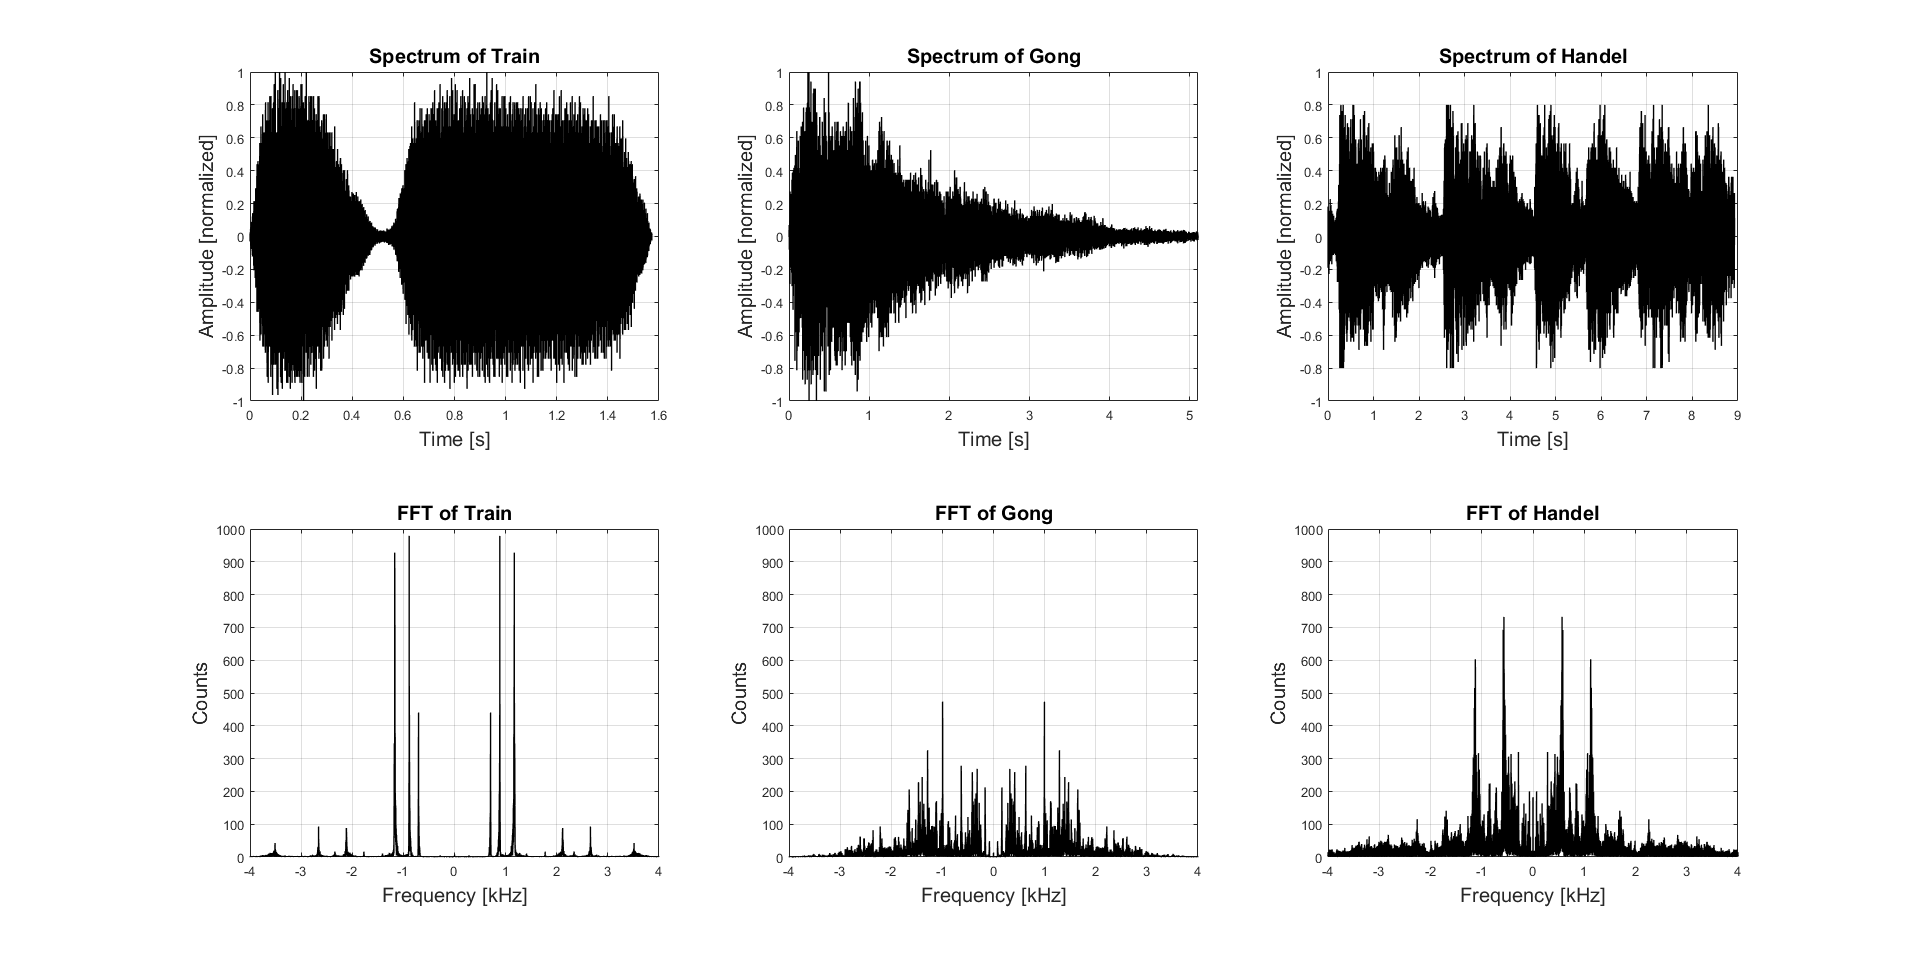
\includegraphics[width=\textwidth]{2.1.png}
		\caption{Time Domain \& Frequency Domain plots of standard MATLAB sounds}
		\label{figure:2_1}
	\end{figure}

	Interesting to note here is that, particularly for the "Handel" file, that the limited sampling rate of the sounds means that no frequencies above 4kHz can be heard when played back. As the clarity in listening applications lies between 14kHz and 20kHz, and the perceived presence of audio around 8-12kHz, you can hear these lacking in the audio files.
		